%!TEX root = ../main.tex
%%%%%%%%%%%%%%%%%%%%%%%%%%%%%%%%%%
% Links:
%
% Difficulty: Companies: 
%%%%%%%%%%%%%%%%%%%%%%%%%%%%%%%%%%

\chapter{Largest square in a binary matrix}
% type of problem why can be useful in real life (image segmentation) dynamic programming
\label{ch:square_in_matrix}
\section*{Introduction}
Imagine you are given a black and white image represented as a boolean matrix of size $N\times M$
where $0$ and $1$ in the matrix correspond to a black and white pixel respectively. Such kind of
image are less uncommon that might be thought at first because they are often the output of digital
image processing algorithms such as masking or thresholding. Further analyzing this kind of images
often requires to identify homogeneous portions of the image. The problem described in this chapter
deals with a simple type of image processing algorithm that involves determining the size of the
largest square area of white pixel of a binary bitmap. We will walk through a number of solutions,
starting from a naive brute-force one, to a more sophisticated, more complex and definitely more
efficine one.
 

\section{Problem statement}
\begin{exercise}
Given a 2D boolean matrix $M$, return the area of the largest square containing only one cells.
	\begin{example}
		\hfill \\
		Given the following matrix the function returns $9$. The largest square has side lenght of
		$3$ and the coordinate of the top-left corner are $(2,1)$. Cells belonging to the largest
		square are highlighted.

		\begin{tabular}{|l|l|l|l|l|}
		\hline
		0 & 0                                  & 1                                  & 1 & 1 \\
		\hline
		0 & 0                                  & 1                                  & 1 & 0 \\
		\hline
		0 & \cellcolor[HTML]{32CB00}\textbf{1} & \cellcolor[HTML]{32CB00}\textbf{1} &
		\cellcolor[HTML]{32CB00}\textbf{1} & 0 \\ \hline
		1 & \cellcolor[HTML]{32CB00}\textbf{1} & \cellcolor[HTML]{32CB00}\textbf{1} &
		\cellcolor[HTML]{32CB00}\textbf{1} & 0 \\ \hline
		1 & \cellcolor[HTML]{32CB00}\textbf{1} & \cellcolor[HTML]{32CB00}\textbf{1} &
		\cellcolor[HTML]{32CB00}\textbf{1} & 0 \\ \hline
		\end{tabular}
		
	\end{example}

	\begin{example}
		\hfill \\
		Given the following matrix the function returns $4$. The side of the largest square is $2$
		and the top-left coordinates are $(2,2)$. Cells belonging to the largest square are
		highlighted.
		\begin{tabular}{|l|l|l|l|l|}
		\hline
		1 & 0 & 1                                  & 0                                  & 0 \\
		\hline
		1 & 0 & \cellcolor[HTML]{32CB00}\textbf{1} & \cellcolor[HTML]{32CB00}\textbf{1} & 1 \\
		\hline
		1 & 1 & \cellcolor[HTML]{32CB00}\textbf{1} & \cellcolor[HTML]{32CB00}\textbf{1} & 1 \\
		\hline
		1 & 0 & 0                                  & 1                                  & 0 \\
		\hline
\end{tabular}

	\end{example}

\end{exercise}


\section{Discussion}
\label{square_in_matrix:sec:discussion}
In the next section we will analyze a number of possible approaches to this problem. We start by
looking at a few brute-force approaches so to then move towards more elaborate and more time and
space efficient dynamic programming solutions

\subsection{Brute-force}
\subsubsection{Incremental side}
\label{square_in_matrix:sec:incremental_side}
The first brute-force approach consists of trying to find the largest square made entirely of set
(i.e. holding a value of $1$) cell by visiting each set cell and by treating it as if it was the
top-left corner of a square. Because calculating the largest square having that cell as top-left
corner is easy the answer to the problem is just the largest value over all the set cells in the
matrix. In order to find out what the value of the largest square having cell $(x,y)$ as top-left
corner we can try build squares of incrementally larger sides around it, starting from side lenght
$1$. At first we try to build a square of size $1$. If that is possible we try size $2$, then $3$,
and so on, until it is impossible or we hit the boundaries of the matrix. The answer for the cell
$(x,y)$ is the last value for a side for which we were able to construct a square. Consider for
instance Figure \ref{fig:square_in_matrix:squa_matrix_incremental} where in order to find the value
of the largest square can be built from cell $(0,1)$, all squares highlighted have to be fully
checked. This approach is clearly correct because eventually we find all squares in the matrix, and
has a complexity of (assuming, with no loss in generality, $N \leq M$) $O(N^4M)$. This is because
there are $O(NM)$ possible starting point for a square, $O(N)$ possible values for the side value
and checking whether a square is valid costs $O(N^2)$ (all cells in the square needs to be checked).
A possible implementation of this idea is shown in the Listing
\ref{list:square_in_matrix:bruteforce1}.


\lstinputlisting[language=c++, caption={Brute force soltuion solution to the \textit{square in matrix} problem using incremental side probing.},label=list:square_in_matrix:bruteforce1]{sources/square_in_matrix/square_in_matrix_solution1.cpp}

\begin{figure}
	\centering
	\label{fig:square_in_matrix:squa_matrix_incremental}
	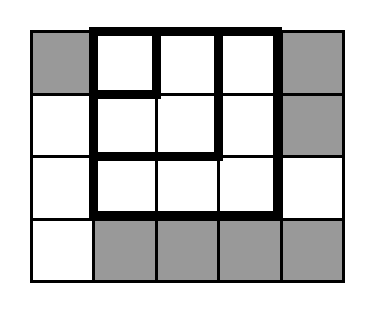
\includegraphics[width=\textwidth/2]{sources/square_in_matrix/images/squa_matrix_incremental}
	\caption[Square in matrix - Brute-force incremental square construction.]{This figure shows  the
	squares that are checked by the brute-force approach for solving the square in matrix problem.
	From the cell $(0,1)$ we first try to build a square of side $2$, and when that is verified to
	be possible, a square of size $3$ is tried. This also succeed and so a square of side $4$ is
	checked, with a negative outcome. Thus $3$ is the largest square having cell $(0,1)$ as top left
	corner. }
\end{figure}

\subsubsection{Walking diagonally}
The idea presented in the Section \ref{square_in_matrix:sec:incremental_side} can be significantly
improved by noticing that is it really not necessary to check, given a cell $(x,y)$ squares of all
possible side lenghts having it as top left corner, fully and one after the other. The idea is that
we can walk diagonally (towards the bottom-right cell) from a cell $(x,y)$ (by incrementing both $x$
and $y$) and, for every step $i$ we take, we check whether all the elements to the left of $(x+i,
y+i)$  and to the right of  $y$ are set, and also whether all the cells in the columns above $(x+i,
y+i)$ and below the cell $(x,y+i)$ are set (see Figure
\ref{fig:square_in_matrix:squa_matrix_diagonal}). If both conditions are true it means that we can
construct a square of side $i$. We can then proceed one step further until a $0$ is found among the
checked cells on the left or above of $(x,y)$. If we were able to perform $t$ diagonal steps, it
means we have found out that the largest square having $(x,y)$ as top-left corner has an area of
$t^2$. The final answer is the largest value we calculated this way across all cell that are set.
See Figure \ref{fig:square_in_matrix:squa_matrix_diagonal} where the numbers represents the cells
that are checked during the corrensponding step. Every highlighted square depicts one of the squares
that is checked by the algorithm.


The time complexity of this approach is $O(N^3M)$, lower than the previous solution. As shown in
Section \ref{square_in_matrix:sec:incremental_side}, there are $O(NM)$ potential top-left corner for
a square and for each of them $O(N)$ diagonal steps. Each diagonal steps costs $O(N)$ as in the
worst case we must check one entire row and column. Thus the complexity of calculating the value of
the largest square having a certain cell  as top-left corner is $O(N^2)$ (See Figure
\ref{fig:square_in_matrix:square_matrix_diagonal} where you can see that no cell is checked twice
during this step). 

Listing \ref{list:square_in_matrix_diagonal} shows a possible implementation of the idea described
here. Note how Listings \ref{list:square_in_matrix_diagonal} and
\ref{list:square_in_matrix:bruteforce1} for both the solutions proposed so far are very similar,
with the only difference being in how the size of the largest square constructible from a certain
top-left cell is computed.

\begin{figure}
	\centering
	\label{fig:square_in_matrix:square_matrix_diagonal}
	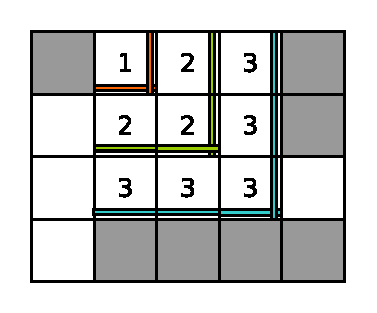
\includegraphics[]{sources/square_in_matrix/images/square_matrix_diagonal}
	\caption[Square in matrix - Brute-force diagonal]{This figure depicts the process of calculating the value of the side of the largest square having as a top-left corner cell $(0,1)$. Each cell is labeled with a number representing the step at which that cell is checked. Note that no cell is checked twice.}
\end{figure}


\lstinputlisting[language=c++, caption={C++ brute force solution using diagonal steps for solving the \textit{square in matrix} problem.  },label=list:square_in_matrix_diagonal]{sources/square_in_matrix/square_in_matrix_solution1.cpp}


\subsection{Dynamic programming}
\subsubsection{General Idea}
\label{sec:square_in_matrix:DP}
Turns out that this problem can be solved faster than $O(N^3M)$ time and in this Section we will see
how with the help of dynamic programming. The gist of the idea is based on the fact for any square
of size $k\times k$ having as bottom-left corner the cell $(x,y)$  has a top, top-left and left
subsquares of size $(k-1)\times (k-1)$. As an example see Figure
\ref{sources/square_in_matrix/images/square_decomposition} which shows a square of size $3\times 3$
decomoposed into $3$, $2\times 2$ subsquares.
\begin{figure}
	\centering
	\label{fig:square_in_matrix:squa_matrix_incremental}
	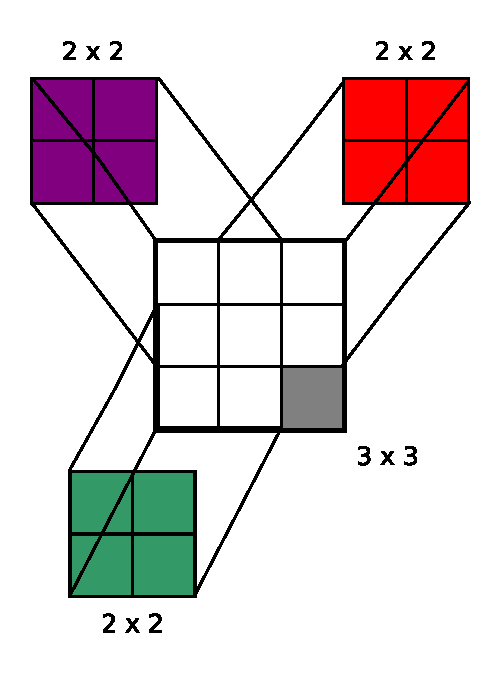
\includegraphics[width=\textwidth/2]{sources/square_in_matrix/images/square_decomposition}
	\caption[Square of side $3$ decomposition into $3$ subsquares of side $2$.]
			{This figure shows how a square of side $3$ can be decomposed into three smaller
	subsquares of side $2$.}.
\end{figure}

Suppose $DP(i,j)$ is a function returning the size of the largest square having the cell $(i,j)$ as
its bottom-right corner (what discussed in this Section can be easily adapted to that $(i,j)$ is the
top-left corner). Clearly the values of $DP(0,j) \: : 0 \leq j \leq M$ (all the cells belonging to
the first row) and $DP(i,0) \: : 0 \leq i \leq N$ (all the cells of the first column) are the same
as the values in the input matrix (either 1 or 0 depending whether on the corresponding value in the
input matrix $M$). This is explained by the fact that a cell in the first row or column lack one or
more of the subsquares described above. For instance for a cell in the first row, the top subsquare
is missing (as there are no cells above it) and thus is impossible to construct a square having a
side larger than $1$ starting from it. For all the other (internal) cells the value of $DP$ can be
easily calculated by using the Equation \ref{eq:square_in_matrix_DPformula}. The formula is
basically stating that if we have a cell $(i,j)$ set to $1$ then, from it we can construct a larger
square whose size depend on the size of the smallest square among the neighboring subsquares.
\begin{equation}
	\label{eq:square_in_matrix_DPformula}
	DP(i,j) = min\{DP(i-1,j),DP(i-1,j-1), DP(i,j-1)\} +1
\end{equation}
Figure \ref{fig:square_in_matrix:square_DP_example} shows the idea above in practice. The value $2$
in $DP(1,3)$, $DP(1,2)$ and $DP(2,2)$ signifies that there is a square of size $2\times 2$ up to
(having that cell as bottom-right corner) those cell in the original matrix. By combining those $3$
squares with the set cell at location $(2,3)$ we can build a larger square of size $3\times 3$. Now
consider the value of $DP(3,4)=3$. The entries for the neighboring cells $DP(3,4)=3$ and $DP(3,4)=3$
implies that a square of side $3\times 3$ exists up to their indices, but the entry at location
$DP(2,4)=1$ indicates that up to that cell only a square of size $1\times 1$ exists and this
prevents cell $(3,4)$ to have a maximum square size larger than $2$ (in other words, making a square
of size $3$ from $(3,4)$ is limited by the cells above it).

\begin{figure}
	\centering
	\label{fig:square_in_matrix:square_DP_example}
	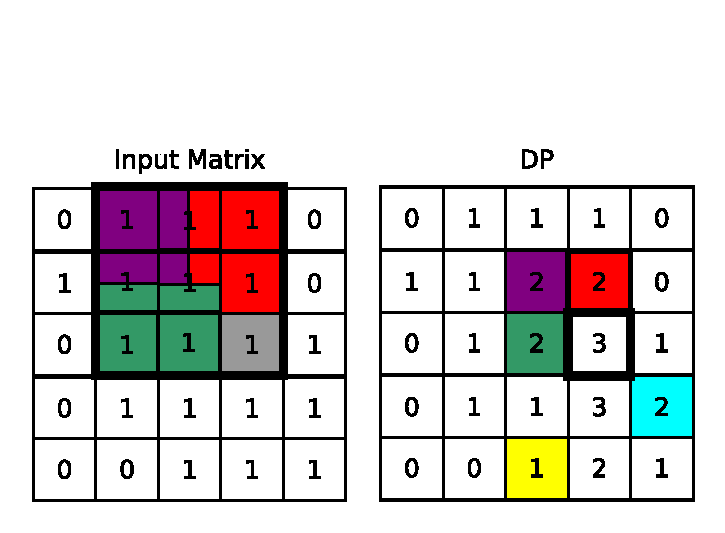
\includegraphics[]{sources/square_in_matrix/images/square_DP_example}
	\caption{This figure shows the values the of each cell in the original matrix and the
	corrensponding values for the largest square having that cell as bottom-right corner. Colors are
	used to highlight the cells that are part of the same square. Note how the cell holding a $3$ in
	the bold frame denote that a square of side $3$ can be constructed from it with cells belonging
	to the top (in red), top-left (purple) and green (right). }
\end{figure}

The function DP in Equation \ref{eq:square_in_matrix_DPformula} is recursive and when drawing its
recursion tree, as shown in Figure \ref{fig:square_in_matrix:recursiontree} (which depicts depicts
part of the recursion tree for $DP(3,3)$),  we can easily see that:
\begin{itemize}
	\item the tree is complete and therefore has an exponential number of nodes.
	\item there are duplicate nodes.
\end{itemize} 
The number of possible unique function calls to DP is bounded by the values of its parameters which
is far less than exponential. In-fact it is proportional to $N \times M$ (the size of the input
matrix) as there are only $N$ possible value for $i$ and $M$ possible values for $j$ in $DP(i,j)$.
Therefore the only way for the recursion tree to have an exponential number of nodes is for some of
them to be duplicates. Given this fact we can conclude that the problem exposes both the property of
\textbf{optimal substructure}, because it can be solved by optimally solve smaller subproblems, and
has \textbf{overlapping subproblems}. Therefore, we can employ dynamic programming and solve each
subproblem only once. In the Sections \ref{sec:square_in_matrix:top_down}
\ref{sec:square_in_matrix:bottom-up} we will go throught the details of the two ways of implementing
dynamic programming algorithm
\begin{itemize}
	\item top-down 
	\item bottom-up
\end{itemize}

\begin{figure}
	\centering
	\label{fig:square_in_matrix:recursiontree}
	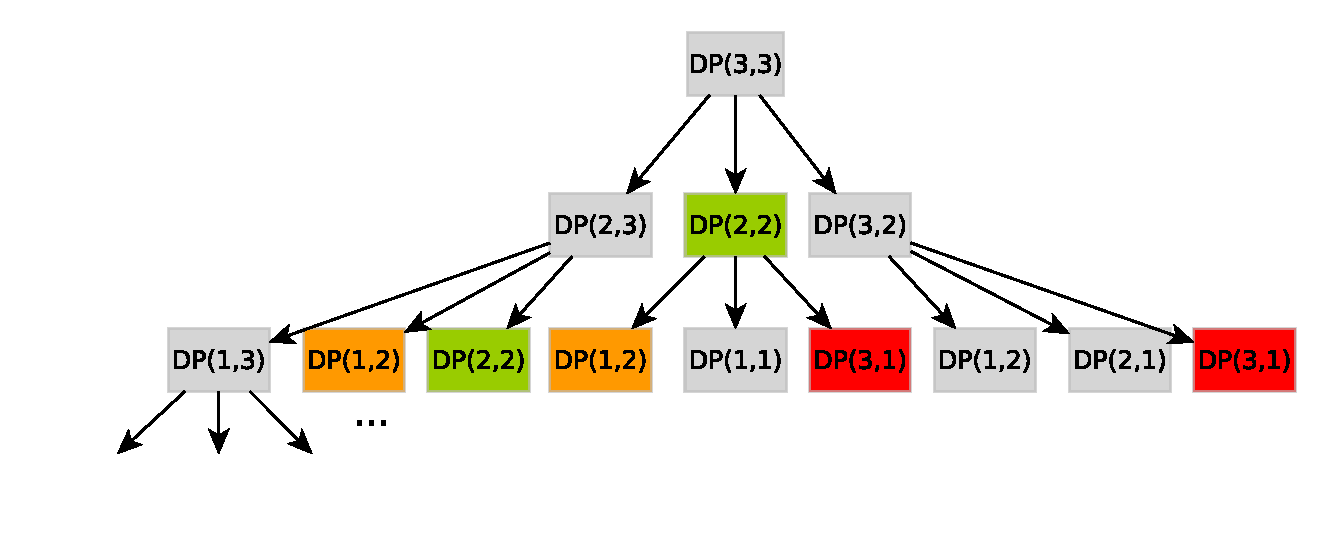
\includegraphics[width=\textwidth]{sources/square_in_matrix/images/recursiontree}
	\caption{This figure is an example of recursion tree for the Equation
	\ref{eq:square_in_matrix_DPformula}. Note that the nodes are duplicates (they are denoted by the
	same color). }
\end{figure}

\subsubsection{Top-Down}
\label{sec:square_in_matrix:top_down}
This is probably the easiest way of implementing the dynamic programming solution for this problem
described in Section \ref{sec:square_in_matrix:DP} as we can translate directly the Equation
\ref{eq:square_in_matrix_DPformula} to a recursive function. The i mpolrtant
trick allowing us to implement it efficiently is to remember the solution
to a subproblem by using a cache (which can easily be a 2D matrix or anything that can allow us to
map $(i,j)$ to a integer, like an hashmap) as shown in Listing
\ref{list:square_in_matrix_top_down}.
As you can see, in the implementation showed here we use as a cache a
\lstinline[columns=fixed]{std::unordered_map<Cell, int>} (where \lstinline[columns=fixed]{Cell} is
just an alias for \lstinline[columns=fixed]{std::tuple<int,int>}) where the functor
\lstinline[columns=fixed]{CellHash}
is the type we provide to \lstinline[columns=fixed]{std::unordere_map} so it knows how to hash a
\lstinline[columns=fixed]{Cell}. The main driver function is the function
\lstinline[columns=fixed]{int maximal_square_in_matrix_top_down(const vector<vector<int>>& matrix)}
which operates in a similar manner as the other solution seen so far, and calculates the final
results by looping over all cells of the matrix and for each of them calculates the largest square
having that cell as a bottom-right corner. The most important part of the code is the recursive
function 
\inline{int maximal_square_in_matrix_top_down_helper( const vector<vector<int>>& matrix,Cache& cache, const Cell cell, const size_t rows, const size_t cols)}
which takes as input the original matrix, the cache (by reference because it
needs to update it along the way) the \inline{Cell} for which it operates on and
the \inline{rows} and \inline{cols} of the input matrix (we are passing it along
so we avoid retrieving it from the \inline{matrix} object for every invokation).

This function which has two bases cases:
\begin{enumerate}
	\item when the current cell has value of $0$ no square can have it as bottom
	right corner, so $0$ is returned.
	\item when we ask for the maximal square from a cell that is outside the
	bounds of the original matrix we simply return $0$. Such cell does not
	exists, so we cannot have a square having it as a bottom-right corner. 
	\item when the value for a cell has been already calculated and it is thus
	already in the \inline{cache} we avoid the expensive work and simply return
	the value in the cache. This is how duplicate work is avoided.
\end{enumerate}
If none of the base-cases conditions are true then, as per the description of
the Equation \ref{eq:square_in_matrix_DPformula}, we calculate the maximal square recursively calling
\inline{maximal_square_in_matrix_top_down_helper} on the cells immediately:
\begin{itemize}
	\item above:\inline{Cell(i-1,j)}
	\item to the left: \inline{Cell(i,j-1)}
	\item to the top-left: \inline{Cell(i-1,j-1)}
\end{itemize}

When the values for all the recursive calls above is finally calculated we save it in the cache before returning it
to the caller so it will be available on subsequent calls.

The complexity of this implementation is $O(NM)$ because the function
\inline{maximal_square_in_matrix_top_down_helper} is executed only $O(NM)$
times (you can verify this by printing the \inline{cell} after the bases cases
in \inline{maximal_square_in_matrix_top_down_helper} and see that no duplicates
appear in the list).


\lstinputlisting[language=c++, caption={C++ dynamic programming top-down solution for solving the
				 \textit{square in matrix} problem. },
				 label=list:square_in_matrix_top_down]{sources/square_in_matrix/square_in_matrix_solution4.cpp}



\subsubsection{Bottom-up}
\label{sec:square_in_matrix:bottom-up}
The other way of implmeneting a dynamic programming algorithm is by using a
bottom-up approach. The idea is in this case to start to filling the cache with
values we know upfront without doing any work. We have already mentioned some of
those values namely the ones beloning to cells of the first row and columns.
Once those values are in the cache we can then proceed calculating the values
for the second row. According to the Equation \ref{eq:square_in_matrix_DPformula} in order to calculate
$DP(1,1)$, the values for $DP(0,1)$, $DP(1,0)$ and $DP(0,0)$ are needed. Because
they all belong to either the first or second row, and because values for cells
in those locations are already in the cache we can calculate $DP(1,1)$. When
$DP(1,1)$ is in the cache, then we can calculate also $DP(1,2)$ and so on for
all the cells in the row. The same reasoning can be applied to the rest of the
rows. Eventually the cache will be filled completely and thus the answer is just
the largest value in the cache. 

Listing \ref{list:square_in_matrix_bottom_up} shows a possible implementation of
such idea.
\lstinputlisting[language=c++, caption={C++ dynamic programming bottom-up solution for solving the
				 \textit{square in matrix} problem. },
label=list:square_in_matrix_bottom_up]{sources/square_in_matrix/square_in_matrix_solution5.cpp}
This implementation initializes the \inline{ans} variable with $1$ or $0$
depending if there is a cell set in the first row or column or not. The rest of
the code loops from the the rest of the cells starting from cell $(1,1)$ and
avoiding the first row and column because as stated before the values for these
cells are known upfront. For each of these cells the final value is calculated
by using Equation \ref{eq:square_in_matrix_DPformula}. 

The complexity is of the code in Linst \ref{list:square_in_matrix_bottom_up} is
clearly $O(NM)$ (probably more obvious in here than in the top-down solution). 


\section{Conclusion}





